\chapter{Конструкторский раздел}

На Рисунке ~\ref{image:scheme} показана структура разрабатываемого проекта.

\begin{enumerate}
\item программа пользователя - программа, использующая ALSA API, определяющая нажатие на гарнитуре
\item специальный файл устройства - создан загружаемым модулем ядра для взаимодействия программы пользователя и модулем ядра.
\item ядро - на этом уровне работает модуль ядра, получающий информацию от программы пользователя через созданный модулем специальный файл устройства.
\item устройство - клавиатура, индикаторы которой будет включать/выключать модуль ядра.
\end{enumerate}

\section{Протокол взаимодействия модуля ядра и программы пользователя}

Для взаимодействия модуля ядра и программы пользователя модулем ядра создан специальный файл, куда программа пользователя будет писать сообщения, а модяль ядра будет обрабатывать эти сообщения.

Сообщение - это нуль-терминированная строка (C-строка или ASCIZ-строка). 

$$N \backslash 0$$ 

Где N - число, означающее номер нажатой кнопки. В данной работе поддерживается только один вид кнопки гарнитуры, поэтому всегда $N = 1$.

\section{Модуль ядра}

Алгоритм действий модуля ядра, при получении сообщения, показан на Рисунке ~\ref{image:alg_module}

\begin{figure}[h]
  \centering
  \includegraphics[scale=0.8]{alg_module.png}
  \caption{Алгоритм работы модуля ядра}
  \label{image:alg_module}
\end{figure}

$msg$ - сообщение из пространства пользователя. Так как поддерживается только один тип кнопки гарнитуры, первый символ сообщения msg сравнивается с единицей.

$my\_tasklet\_function$ - функция отложенного действия, запускающая первый раз таймер с функцией, изменяющей состояние LED индикатора клавиатуры.

Алгоритм отложенного действия показан на Рисунке ~\ref{image:alg_tasklet}

\begin{figure}[h]
  \centering
  \includegraphics[scale=0.8]{alg_tasklet.png}
  \caption{Алгоритм отложенного действия}
  \label{image:alg_tasklet}
\end{figure}

$my\_timer\_func$ - функция, изменяющая состояние LED индикатора клавиатуры.

$sos$ - массив числел, означающими длительность включения индиктора клавиатуры.

$pos$ - текущий индекс массива $sos$.

$run$ - флаг, означающий, что в данный момент сообщение sos еще выполняется.

Но последовательность действий \ref{panic} может привести к печальным последствиям, если после выполнения строчки №3 и до выполнения строчки №4 Linux решит прекратить выполнение данного кода, и начнет выполнение другой задачи. Этой другой задачей м.~б. этот же код. Тогда возможна ситуация, когда в ядре активны оба процесса, которые считают, что они выполняются в единственном экземпляре. Так как я ядре этот код работает с аппаратурой, то одновременное выполнение одной и той же программы приведет к kernel panic. 

\begin{lstlisting}[language=C,caption={Опасный код},label=panic]
if (run > 0) {
  return ;
}
run++;
...
\end{lstlisting}

Алгоритм функции таймера показан на Рисунке ~\ref{image:alg_timer}

\begin{figure}[h]
  \centering
  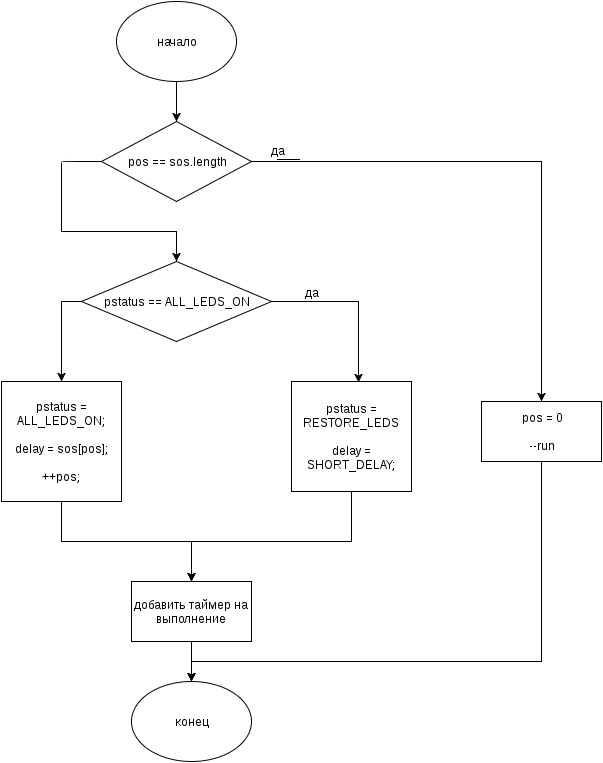
\includegraphics[scale=0.8]{alg_timer.png}
  \caption{Алгоритм функции таймера}
  \label{image:alg_timer}
\end{figure}

$pstatus$ - флаг включения индикатора клавиатуры.



